\documentclass[]{article}
\usepackage{multicol}
\usepackage[margin = 1.25in]{geometry}
\usepackage{graphicx}
\usepackage{mathtools}
\usepackage{caption}
\usepackage{lipsum}
\usepackage{algpseudocode}
\usepackage{fancyvrb}
\usepackage{amsfonts}
\usepackage{amsmath}
\newenvironment{Figure}
  {\par\medskip\noindent\minipage{\linewidth}}
  {\endminipage\par\medskip}

\linespread{2.0}
\setlength{\parskip}{1em}

\newtheorem{theorem}{Theorem}[section]
\newtheorem{lemma}[theorem]{Lemma}
\newtheorem{proposition}[theorem]{Proposition}
\newtheorem{corollary}[theorem]{Corollary}

\newenvironment{proof}[1][Proof]{\begin{trivlist}
\item[\hskip \labelsep {\bfseries #1}]}{\end{trivlist}}
\newenvironment{definition}[1][Definition]{\begin{trivlist}
\item[\hskip \labelsep {\bfseries #1}]}{\end{trivlist}}
\newenvironment{example}[1][Example]{\begin{trivlist}
\item[\hskip \labelsep {\bfseries #1}]}{\end{trivlist}}
\newenvironment{remark}[1][Remark]{\begin{trivlist}
\item[\hskip \labelsep {\bfseries #1}]}{\end{trivlist}}

\newtheorem{hyp}{Hypothesis}

\makeatletter
\newcounter{subhyp} 
\let\savedc@hyp\c@hyp
\newenvironment{subhyp}
 {%
  \setcounter{subhyp}{0}%
  \stepcounter{hyp}%
  \edef\saved@hyp{\thehyp}% Save the current value of hyp
  \let\c@hyp\c@subhyp     % Now hyp is subhyp
  \renewcommand{\thehyp}{\saved@hyp\alph{hyp}}%
 }
 {}
\newcommand{\normhyp}{%
  \let\c@hyp\savedc@hyp % revert to the old one
  \renewcommand\thehyp{\arabic{hyp}}%
} 
\makeatother


%opening
\title{Modeling Network User Behavior: Probabilistic Programming and Beyond}
\date{May 13, 2016}
\author{Shidan Xu}


\begin{document}
\maketitle

%\begin{abstract}
%
%\end{abstract}



\section{Abstract}

This paper describes a Master of Engineering project at the MIT Advanced Networks Architecture (ANA) group. This project involves learning to predict users' mobility within the network topology. This topological mobility, as opposed to physical mobility, can be substantial as the user switches from LTE to wireless network, while moving minimally physically. Our dataset consists of email IMAP logs as they document associated client IP addresses, as well as the clients' identifiers. Prediction for online mobility is of particular interest to the networks community. If we can predict online mobility with high probability, then new network architecture can be designed to optimize the caching system by minimizing resending packets.  We used various approaches and techniques to model the user's behavior, including probabilistic programming, regression, neural nets, and clustering algorithms. We compare and contrast how different models differ in their prediction accuracy, speed of convergence, and complexity. 


%This paper describes a thesis project at the MIT Advanced Networks Architecture (ANA) group. This project involves predicting a user's behavior in various networks. In particular, we are interested in how the user is likely to transition between networks. We plan to design various models to predict the user's behavior, and use various evaluation criteria to understand which model most vividly captures the user's behavior. As a learning experience for our team and me, we employ probabilistic programming (PP) techniques. PP is a way of programming that utilizes existing software packages that include encapsulated methods for the inference step of machine learning. By simplifying the implementation, it allows researchers to focus on models. This project has two main objectives. The first is to design several models to capture one or multiple aspects of a typical user, or a group of users' behavior in a network. The second is to evaluate each model to decide which model is more feasible, and which model is applicable under what situations. Together this project aims to give a better understanding of how network user transitions.

\newpage
\section{Introduction}

Noam Chomsky believed that the Merge operation is one of the fundamental differences that separate humans apart from other primates \cite{whyonlyus}. That is, humans can take two abstract concepts and combine them to create scenarios that s/he has never physically experienced. A person can imagine a dinosaur ripping apart an opera stage as long as he understands dinosaurs and opera, despite he has never seen such an event in reality. This Merge ability can induce creativity. In the networks community, research on evaluation of network architecture is sometimes qualitative (SOURCE?). Statistical methods and machine learning are trending approaches to extract insight out of the dataset. By applying machine learning strategies to a networks problem, we try to develop new insight that's not traditionally seen.

This project relates to the FIND (Future Internet Design) initiative \cite{find}, which asks the question of what the requirements should be for a global network 15 years from now, and how we can build such a network if we are not constrained by the current Internet. Developers of the Internet made some design choices with assumptions. One particular assumption is that network mobility is similar to mobility in geography\cite{jacobson}. However, in real world cases, we found that assumption to be sometimes violated. For example, a user could transition from a 4G network to Wi-Fi by walking a few meters in real world, but the IP addresses in network topology are likely to be not adjacent, even entirely different. In extreme cases, the nearest common ancestor of nodes in network topology can be on opposite coasts of the country. Such design is costly for the user to transition between networks. In designing a new network, one of the focal points is to decrease such inconsistency, as packets of information need to be rerouted.

Imagine one typical 9-5 worker. She wakes up at 8, goes to work at 9, comes home at 5. She has dinner at 6 and spends two hours surfing the web at night. Now imagine how her daily network usage would look like. She would be on her home network in the morning. She uses a combination of the company and LTE network at work. Sometimes she eats lunch at a coffee shop and uses the network there. She spends some time on her home network at night. Her active network traffic ends at 11, but some passive email checking and other maintenance from her device persist throughout the night. Her daily network usage is very predictable. If researchers can predict her network usage, notifications can be customized to make her life more convenient. 

Imagine another person traversing through a college campus while checking his email on the phone. As he moves along, his phone?s network switches from LTE and his college network alternatively. Every time the user switches network, his phone loses some data and has to send extra requests to recover lost data. The LTE and campus wifi, despite being geologically close by, can be vastly distant in network topology. Hence a request may have to go up multiple layers, before finally reaching a common ancestor. This extra path traversed carries inefficiency in the current network. 

Multiple questions can be asked in those two scenarios. To what accuracy is human network behavior habitual? To what degree can network behavior be predicted? How should we evaluate network usage behavior? How often do such costly network transitions happen? How do we measure the cost of one such transition? How should we design our networks to avoid this costly transition?

This project focuses on understanding the users. We believe that the networks serves the users, not vice versa. Additionally, the project stresses to create a procedure for quick turnaround of modeling using approaches such as probabilistic programming and neural nets. These procedures are chosen to quickly expand on the current model. The researcher spent time in evaluating the different approaches and tools for their performance. 

\newpage

\section{Related Works}

A major related paper to this particular project is Yang's Measurement and Modeling of User Transition Among Networks \cite{yang}. This paper created one particular 3-state hidden Markov model that's evaluated by measuring the distribution of cost function of signaling a network attachment / detachment. While the paper serves as a decent exploration baseline, we explore deeper on some aspects, definitions, and assumptions. For instance, the Yang paper assumed all users form one uniform group. We expand the work by including several clustered user classes. We expand the work in the modeling space. Note that the Yang paper created a Markov model that is not easily expandable. If another factor is identified to be significant, the entire modeling process needs to reinitiate. We want to avoid such inefficiency in further modeling, by utilizing tools and techniques that facilitate exploration in modeling space.

There are a few related works in applying machine learning to a networks problem. In Beverly \cite{beverly}, the author described several learning approaches for attacking various networks traffic problems with minimal dataset. In particular, learning was useful in capitalizing on under-utilized information and inferring behavior reliably. Using a hidden Markov model, Beverly was able to infer TCP congestion based on the IP address bits. Beverly's view agrees with our viewpoint that statistics and machine learning can provide extra insight into the dataset. By utilizing statistical methods to aid humans in extracting the intricacies of data, we improve inference performance.

Probabilistic programming is a generative learning approach, and an ongoing research area. Generative learning approaches can analyze complex scenes more richly and flexibly, but have been less widely embraced due to their slow inference speed and problem specific engineering to obtain robust results \cite{kulkarni}. One of the trending topics lately in probabilistic programming is in creating a generic inference engine that facilitates optimization of parameters.  This inference engine facilitates code implementation for different models. Many current applications are under developed for probabilistic programming. Picture and Venture are two such probabilistic programming languages conceived at MIT. Both languages focus on the development of a general inference engine. With an inference engine, a user can take the benefit of probabilistic models without having the the expertise in statistics. We refrained from using those languages as they are alpha versions and are standalone platforms that have higher learning curves. Instead, we explored PyMC3, a stable python package that's written with a general inference engine. We chose this option because we want to explore more models without having to implement the inference methods ourselves \cite{ghah}. 

In Tenenbaum \cite{tenenbaum}, current applications and limitations for probabilistic programming are discussed, with a vision for hierarchical structural learning. In hierarchical structural learning, the algorithm can learn the dependence of variables. That is, not only can the learning algorithm optimize the parameters for the model, it can also learn the most appropriate structure of the model. With enhanced storage capacities and computational cheapness, hierarchical structural learning can facilitate data mining further by saving the scientists time to conceive the most logical model.

\newpage


\section{Modeling}
\subsection{Dataset}

To understand user behavior across networks, we have several options for picking our dataset.

????????????? ?yang??????? ????????????? ???? ??user??? ???

The ideal option is to have all willing users to install a software on all of their connection devices to collect measurement data. Such user population is difficult to find and manage, and such monitoring drains the device battery \cite{yang}.
  
\begin{itemize}
\item
Email logs
\item
Eh...
\end{itemize}

Multiple datasets exist for carrying out this research. We decided to first reproduce the Yang paper \cite{yang} results as a baseline. Hence we worked with the UMass dataset. The UMass dataset contains user email activity in the form of IMAP logs for residents of University of Massachusetts at Amherst. The dataset includes user information such as the identity, the time of action, and action in terms of attaching to network, detaching from network, IP address, and the device used to log in. The Yang paper built a three-state Markov model for evaluating user transitions. That is, 

????imap logs????????? ???????????????

With this information, we can decide whether a transition happens from the logs. Brian Copeland, a UROP student of the group, parsed the original log entries into SQL entries that contain each individual session, or duration when the user is on a particular network. We overlay the durations to decide occurrences of transition. The details of transition criteria can be found in Yang \cite{yang} paper.

????????? ??????????? ??????????????
??? ????
?????
???
device???????


To understand how users make network transitions, first we need to define a transition.

\begin{definition}
A \textbf{session} is a continuous period of time for which a user is on the same network, which is defined by the same IP address. A \textbf{transition} happens when the user detaches from one network and attaches to another one.
\end{definition}

In reality, the user is often simultaneously on multiple networks thanks to the multiple devices s/he owns. So we looked at each 15 minute windows. We look at the networks the user is on at the end of the 15 minute window, versus at the beginning, to see whether s/he has transitioned. 

\subsection{Questions}

The first step in creating an efficient network is to understand the users. We can ask several major questions: 

\begin{itemize}
\item
Can the entire user population be broken down into groups? How many different groups of users are there? 
\item
How frequently do users transition? What does a typical transition look like?
\item
Do users exhibit any periodical behavioral patterns?
\end{itemize}

To answer questions above, we continue to modeling.

% This chapter can be redone by starting from a markov model approach, then explain the ups and downs that lead to 

The approaches used here are

\begin{itemize}
\item
Markov Model
\item
Regression
\item
Probabilistic Programming
\item
Clustering
\end{itemize}

\subsection{Markov Model}

\begin{center}
    \begin{tabular}{| l | l | l | l |}
    \hline
     Transition Prob.& On 0 Networks & On 1 Network & On $>=1$ Networks\\ 
    \hline
    On 0 Networks CRF& 0.905 &0.088 & 0.007\\ 
    On 1 Network& 0.587 &0.352 & 0.061\\ 
    On $>=1$ Networks & 0.209 & 0.322 & 0.469\\
    \hline
    \end{tabular}
\captionof{table}{Empirical estimates of transition probabilities. Data acquired on training sample (1000 user days).}
\end{center}

In Yang \cite{yang}, the researchers provided a three-state hidden Markov model to count the number of transitions. We started out by reproducing this approach. We model the user in three states: not on a network, on one network, on multiple networks. A 3 by 3-state transition matrix can be calculated directly from the dataset. We take measurements at the end of each 15-minute period. In table 1, we have the transition probability matrix calculated on a 1000 user days training sample. Given this transition probability matrix, we can generate estimations of what the user may behave in the future. We do not believe that such modeling optimally captures user behavior for the following reasons.

\begin{itemize}
\item
Loss of information by the probability matrix.

By categorizing the user into one of the three states, we assume the transition only depends on the number of networks a user is on. The user's likelihood to make a transition can depend on other factors, such as how long s/he spends time on the current network.

\item
Loss of individuality of users

The entire dataset contains users of various habitual patterns. There could be a number of groups of users who have contrasting transition probability matrix. By combining all users together, we only gain insight on how an "average user" behaves like, though this "average user" may be a mix of several exemplary users.

\end{itemize}

For baseline, we evaluate the distribution of the number of transitions for all users on a daily basis as noted in Yang. We identify a transition as a change of state (on 0, on 1, or on 2 or more) from the end of the previous 15 minute period to the end of the current 15 minute period. We compute one distribution from the testing dataset, and another for the randomly generated dataset based on HMM runs. We make the simple assumption that all users behave similarly and the transition distributions are approximately normal. 

\begin{Figure}
 \centering
 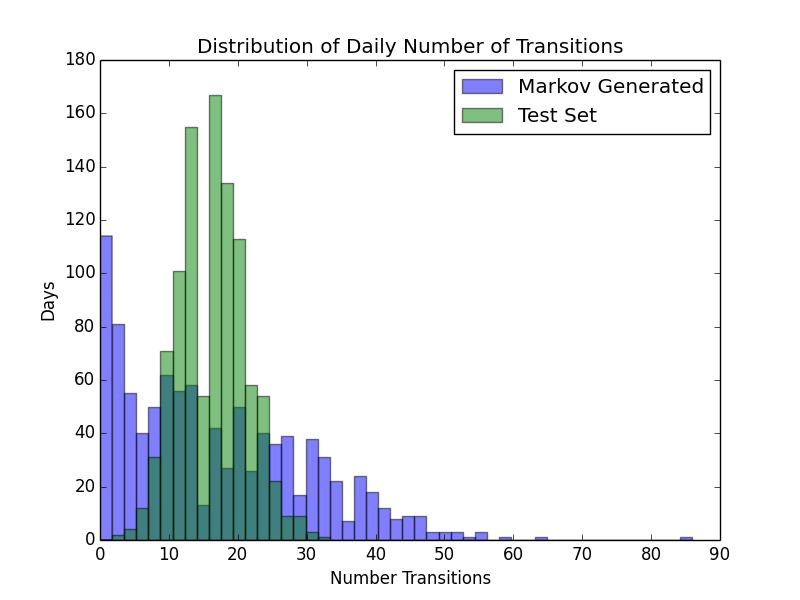
\includegraphics[height = 11cm, width =15cm]{figure_1.png}
 \captionof{figure}{The distribution of number of transitions from HMM and testing set. Sample size 1000 user days each.}
\end{Figure}

In figure 1, we illustrate the distribution of daily transitions for 1000 sample days generated by the HMM and 1000 days from the testing data. The testing data shows a more Gaussian distribution, whereas the HMM generated data shows a skewed tail. Despite the two datasets having similar transition probability matrices, the HMM failed to capture the normal distribution. We confirm the concern that a simple three state Markov transition matrix alone does not perfectly capture the transition behavior exhibited by the dataset.

We need some modeling technique that can once an for all finish everything. 


\subsection{Regression}

To answer the question how frequently do users transition, there are several parameters we can model. We chose to model for each user, how many sessions happened in a given day, and what is the duration of each session. If we can accurately model the number of sessions in a day and when exactly these sessions happen, then we can overlay the sessions to evaluate the transitions.

Here a regression model was used to predict the number of sessions of each user per day. Since each user is different, we tried three approaches: 
\begin{itemize}
\item
Treat all users as a uniform group. 
\item
Cluster users as user groups.
\item
Treat each user as a separate entity.
\end{itemize}

Two types of regression were examined, namely Ridge regression and Logistic regression. Ridge regression is a evaluation with alpha penalty on norm of weights. Logistic regression is a classifier where the output is categorical. We used a linear model for both regressions.

First we look at the general user population. We used scikit-learn as our library, for its ease of use and availability of tutorials. We passed in 5 million entries of session data, where each entry $x_i$ consists of user ID, IP address by bits (32 bits), timeStartBucket \{0 - 23\}, day of week, device, whether the device is Apple, and whether the device is Android. For Ridge regression each $y_i$ is the duration of the session. For Logistic regression we further broke duration into short ( $<$ 5s), mid (5s - 60 mins), and long ( $>$ 60 mins). The cutoff at 60 minutes is because we noticed a peak at slightly more than 60 minutes for duration distributions.

\begin{Figure}
 \centering
 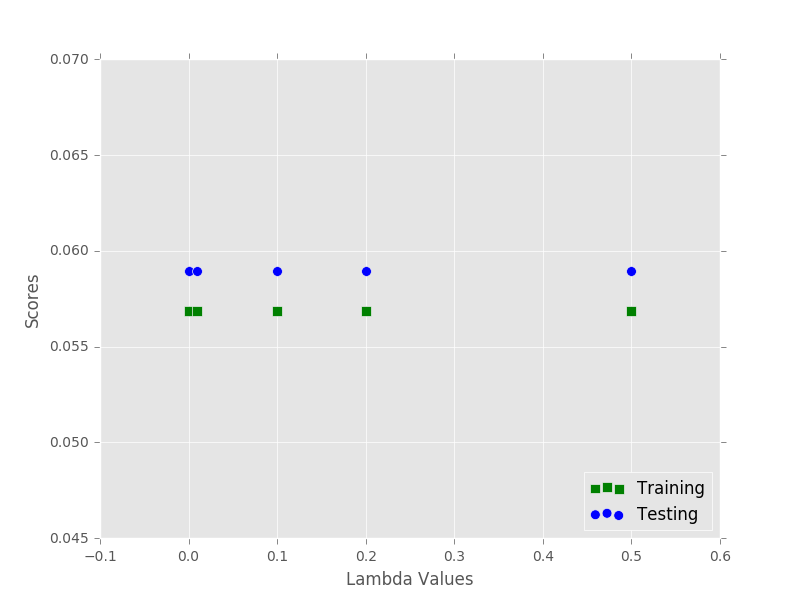
\includegraphics[height = 7cm, width =10cm]{ridgeScores.png}
 \captionof{figure}{Ridge Regression Scores.}
\end{Figure}

Using this dataset to train, we tried to make predictions on the session duration of the remaining 2.5 million available entries. Unfortunately, we reached terrible scores ($<10\%$) for Ridge regression. This is largely due to the secondary peak at the hour mark. Our features do not have ability to distinguish whether a duration is going to be less than a minute or an hour long. Because the prediction is linear, the results easily becomes bizarrely off.

\begin{Figure}
 \centering
 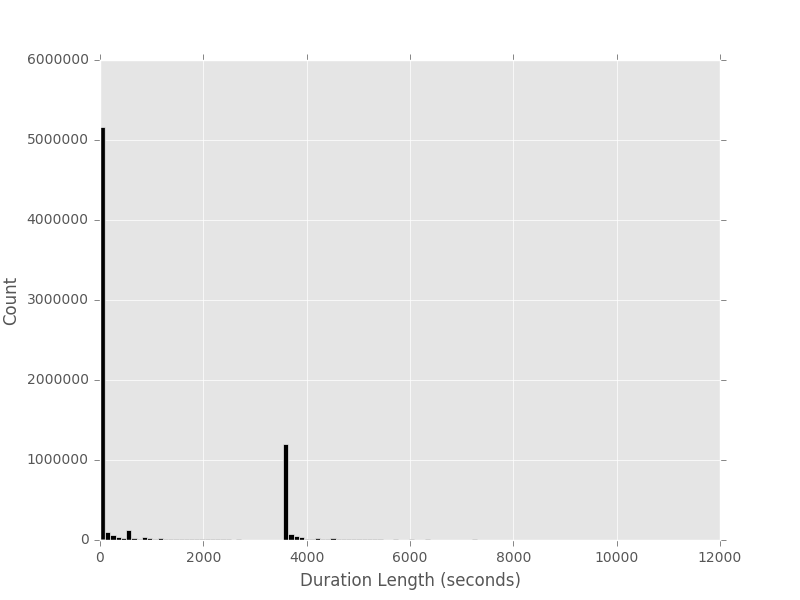
\includegraphics[height = 7cm, width =10cm]{durationDistribution.png}
 \captionof{figure}{The distribution of session durations, in seconds. Note the second peak at the hour mark.}
\end{Figure}

The Logistic regression predicts correctly the duration tag(long, mid, short) at $67\%$ accuracy, which is better than chance (1/3). Those values are far from accurate predictions. The features that carry the most weights are Apple or Android, and specific leading bits of the IP address. Having the device being Android gives a +1.2 weight for producing a long session.


[Extend to newly appended dataset and do it per user group, per user]

\subsection{Neural Net}

Due to the bad performance of regression, we decided to do the same task with a simple one hidden layer neural net. With aid from Python's Theano library, we implemented a neural net with 5 features, 3 output nodes, and 10 hidden nodes. This net correctly predicts the duration tag with 95\% accuracy. This increment in performance may be partly due to the hidden nodes in the neural net can better express the unknown relations that were constrained by the limited number of features we provided.

[Include image on neural net output]

\subsection{Bayesian Modeling and Probabilistic Programming}
\subsubsection{Generative vs. Descriptive Modeling}

Despite the neural net having a high performance, we note that neural net is mostly a classifier. That is, such an algorithm is an example of a descriptive algorithm. In general, modeling algorithms can be classified into two categories, generative vs. discriminative. A discriminative algorithm learns what criteria separate the classes given the dataset.  For instance, logistic regression is a discriminative algorithm. A generative model, focuses on each class, and creates a model for what the underlying process for each class is \cite{ng}. Let $x$ be the feature inputs to the model, $y$ be the model output prediction, discriminative models learn $Pr(y | x)$, whereas generative models learn $Pr(x | y)$. Therefore, generative model allows researchers to synthesize new dataset by understanding what the underlying distribution is. The Markov model is a generative approach, whereas regressions and neural nets are mostly descriptive models. We used the the discriminative approach when we needed to correctly classify or quantify parameters, and used generative approaches when predicting future actions.

\subsubsection{Probabilistic Programming}

In this project we explored modeling using probabilistic programming, a kind of Bayesian modeling. Bayesian modeling creates a prior belief of how data \textit{should} look like before actually inspecting the dataset. Then, given the dataset, we produce a distribution for each parameter that we are interested in estimating, i.e. the posterior distribution \cite{ppblog}. Probabilistic programming is a way of inferring the ideal parameters for such modeling practice. It is a programming language as it abstracts away the mathematical calculations that goes on in inferencing the optimal parameters, just like a typical programming language abstracts away the storage of pointers in memory.

Roughly speaking, the steps involved in probabilistic programming are as follows:
\begin{itemize}
\item
Declare prior beliefs on what the data looks like.
\item
Feed in dataset.
\item
A sampling algorithm calculates a posterior distribution for each parameter in the model.
\end{itemize}

Probabilistic programming languages enable you to state your priors beliefs and your model with elegant, statistical syntax. Typically, the larger the dataset that's feed in, the less significant the prior beliefs become for learning the final parameters. In rare cases, the initial setup can produce local optimum that is impossible to climb out of. Hence it is recommended to examine several different prior beliefs. 

PP represents data and distributions with probabilistic parameters. Using a probabilistic programming approach gives estimation for parameters such as the mean of the normal distribution in distributions, as opposed to exact values. So PP makes statements such as "The mean of the normal distribution is normally distributed around 14 with a variance of 3.", instead of "the mean of the normal distribution is 14". This is beneficial as it can better capture the variance and other characteristics of shape.

We implemented a five factor model using probabilistic programming. Essentially, we are predicting two things, the number of sessions in a day, and the duration of an average session. We used Python PYMC3 as our API library. PYMC3 uses next-generation Markov Chain Monte Carlo sampling algorithms such as the No-U-Turn Sampler (NUTS) to sample its probability distribution \cite{pymc3}. Essentially, it constructs a Markov Chain that has the desired distribution at its equilibrium distribution, and uses Monte Carlo simulations to reach the approximation equilibrium. We can think of MCMC as similar to stochastic gradient descent in neural nets, which is a way of estimating the optimal parameters for the distribution. 

The pros for using PYMC3 include fast inference engine and simplicity to switch between distributions. PYMC3 offers NUTS and Hamiltonian Monte Carlo sampling, which works well on high dimensional and complex posterior distributions and allows complex models to be fit without specialized knowledge on fitting algorithms \cite{pymc3}. For instance, one can easily model the start time for each session as a normal distribution in PYMC3. Later, if one decides that a exponential distribution fits better, s/he can easily specify the desired shape for start time again.

\begin{Figure}
 \centering
 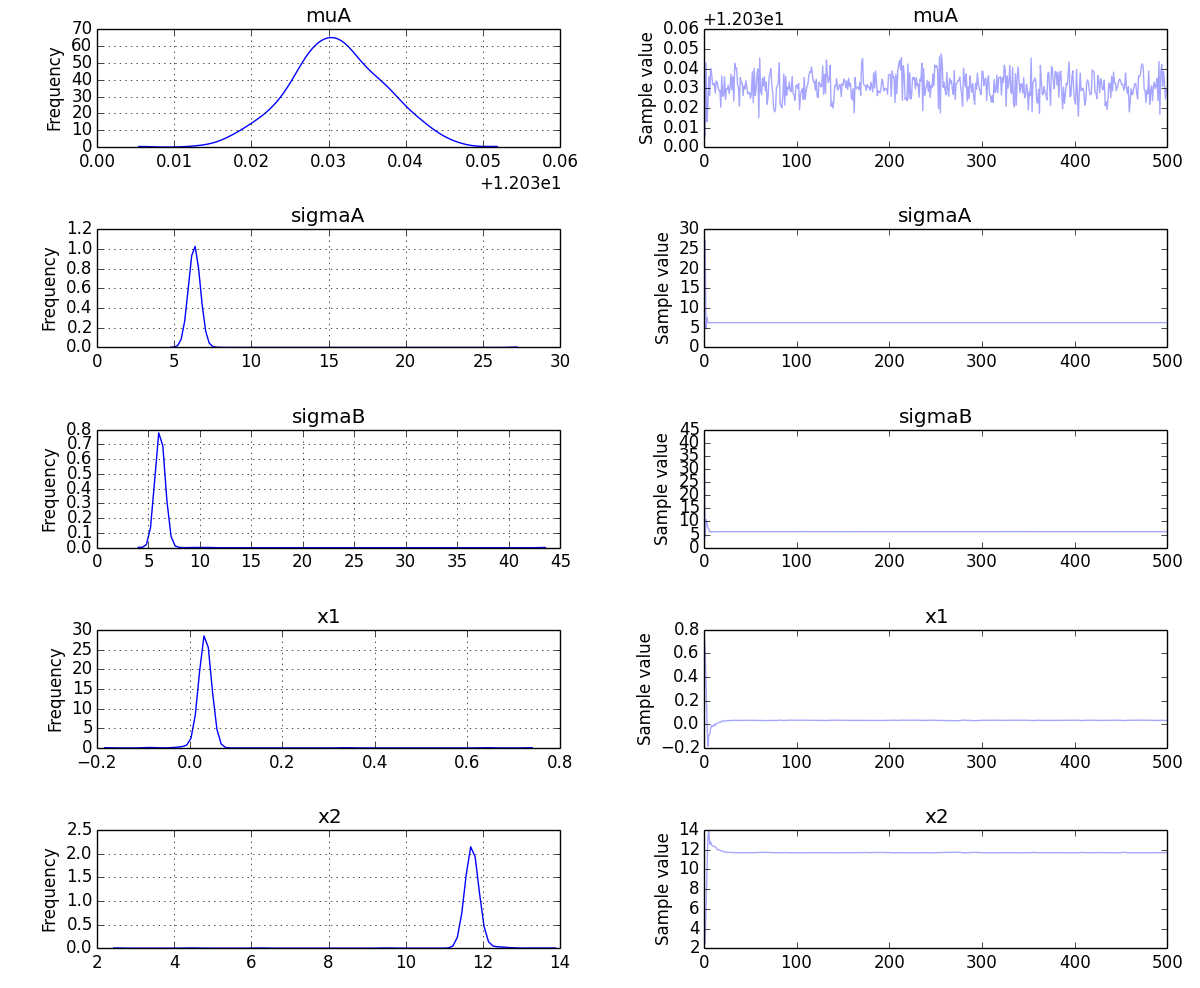
\includegraphics[height = 10cm, width =12cm]{ppsample.png}
 \captionof{figure}{An example PP output using PYMC3. A is the distribution of start times of a typical session, which is modeled as normal. We see that the mean is normally distributed around 12.033 with $\sigma$ of approximately 6. The right column shows each sampled $\mu$ and $\sigma$ values over the 500 sample Monte Carlo trials.}
\end{Figure}


With this approach, we implemented a duration prediction as a combination of two normal distributions, with a switch point. Switch point happened at 1800s, where the later normal has mean 3466 second, the earlier normal has mean 3.53 seconds. This approach is done on the general user population, hence it remains unclear what exactly are the factors that can cause the switch between long and short durations. 

Notably, we spent a lot of time in vein tweaking around the API to analyze more sophisticated, multiply dependent models. Please see challenges to see the lessons learnt related to PYMC3 and probabilistic programming.

\subsection{Clustering}

A closer inspection at the dataset conceives the idea that we may split the user into user groups. The population in the dataset is residents of UMass. This could include professors, students, and other populations whose behavioral pattern are vastly different. It would be beneficial for the algorithm to take separate inferences for each one of the groups. We used K-means analysis for carrying out the clustering analysis. K-means analysis picks the $k$ initial starting centroids for the population, and gradually update the position of centers as the algorithm iterates itself. In Tibshirani\cite{tibshirani}, the optimal number of clusters $k$ can be found using the gap statistic. We implemented such an algorithm with features including ID, IP, start time, end time, duration, Android, Apple, device. We found three clusters in total. This clustering separates the users mainly by durations. 

\begin{Figure}
 \centering
 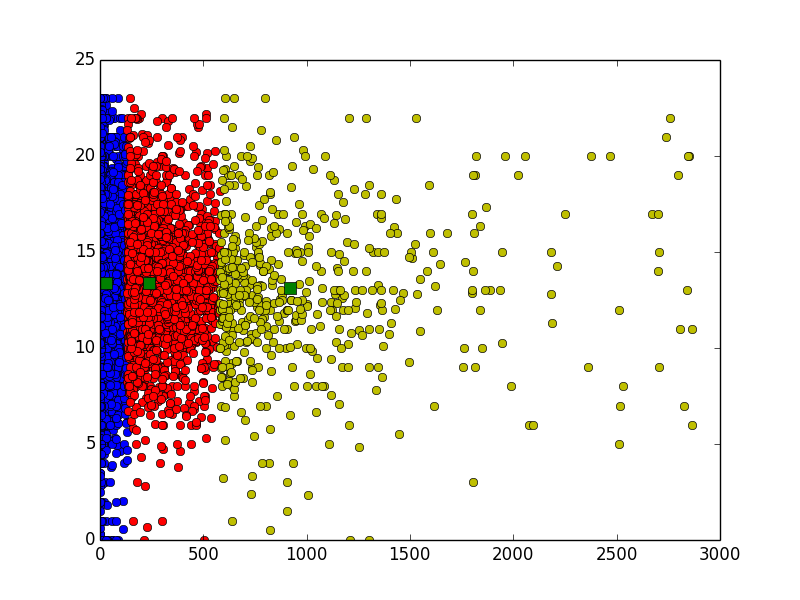
\includegraphics[height = 9cm, width =12cm]{3ClusterKMeans.png}
 \captionof{figure}{The clustering algorithm output. X-axis is duration in seconds. Y-axis is session start hour. Those were two of the features that affected the clustering. The green dots represent the centers of each cluster.}
\end{Figure}

\begin{Figure}
 \centering
 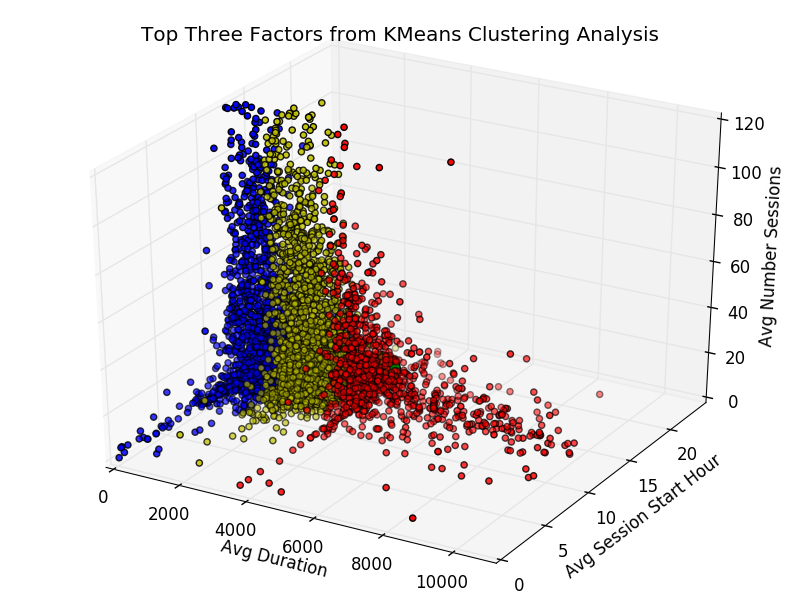
\includegraphics[height = 9cm, width =12cm]{Threefactorclustering.png}
 \captionof{figure}{The K-means clustering algorithm output. The top three factors for separating the dataset are average duration per session, average number of sessions in one day, and the average starting hour for sessions.}
\end{Figure}

A K-means clustering algorithm helps quantify the influence each feature has on dissecting the dataset. Here the k-means algorithm proposes that average session duration is the number one factor for distinguishing user types. Another plausible but less promising factor is the average number of sessions on an average day.

The researcher makes the following arguments and observations regarding this output.

\begin{itemize}
\item
Users with on average long durations may be less likely to transition.
\item
The number of sessions per day can directly affect the calculation of how frequently the user transitions.
\item
Users who have on average short sessions and high number of transitions tend to switch between networks more frequently. Hence when designing a new network to maximize efficiency, those users deserve extra attention for congestion.
\end{itemize} 

We move on to test the arguments above.

\subsection{Canonical User}

To test out the hypotheses above, we break the users into clusters, and then calculate the Markov transition probability matrix to see whether there is a significant difference.

\begin{hyp}
The average user in the long duration cluster exhibits on average less number of transitions than the average user.
\end{hyp}

$H_0$ is that the average user in the long duration cluster exhibits on average the same number of transitions as the average user.

First we see that on average, the long duration cluster has a daily 18.49 sessions, whereas the average user has a daily 20.64 sessions.

\begin{Figure}
\centering
 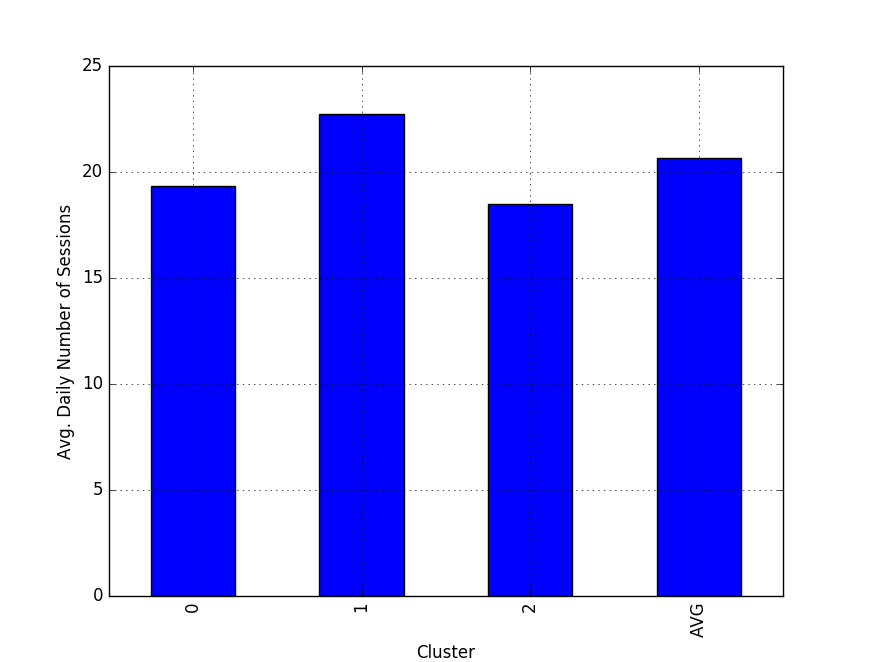
\includegraphics[height = 6cm, width =9cm]{clusteredAVGNUMSESSION.png}
 \captionof{figure}{The average number of sessions per cluster.}
\end{Figure}

After calculating transitions as defined in section 4.1, we obtain the following results.

[Include the graph on transitions]

[Here a better figure would be at least three dimensional and takes the top three factors.]

[This part needs to be redone and at least triply expanded since the clustering is done on users. We can do better by more clearly include more features and separate by users' averages]

\newpage
\section{Evaluation}

\subsection{Approach Comparison}

This project gives the author a much more thorough understanding on what approaches are plausible for a networks dataset. In general, a sophisticated neural net requires relatively thick datasets. That is, for each entry, we need more features than the available 10. 

A sophisticated neural net still remains the most fruitful approach. However a neural net decreases the importance of human decision in creating the models. If the human has no idea what is happening in the dataset, then a neural net may better assist him to explore the undiscovered possibilities. However, such an approach does not tell causation apart from correlation. Two features may be both positively affecting a tag, but really one of the two causes the other and the positivity of the tag. So, if we use a graphical model approach, i.e. bayesian probabilistic approach, the researcher can better specify the details of the models. 

Regressions, whether Ridge or logistic, trades speed for prediction accuracy. A typical regression finishes in less than 30 seconds, whereas training of a million entries in a neural net can take up to [IDK, half an hour, try again to be precise.] 

In all the approaches we took, we treated the models no more complex than a linear model. Ceteris paribus, we see that neural nets perform the best because it introduces hidden layers and extra parameters. This suggests that in all trainings we did, we did not have enough features and parameters to correctly tune for the results. The fundamental difference in the different approaches we take involve how much we understand the dataset. The specific probabilistic programming we did requires knowledge on the structure of the dataset. We need to additionally understand the structural dependence of the parameters.

This is somewhat due to the width of our dataset. For each entry, we have at most 10 parameters. Those 10 parameters do not necessarily have enough decision power over the prediction values we wanted to predict. Therefore, a neural net may be a better approach, as it introduces enough hidden parameters. Alternatively, we could introduce hidden intermediate nodes in the graphical models and connect them with corresponding nodes. However, such an approach proves to be overly complex beyond PYMC3 abilities. 

[This should be a large section]

\newpage
\section{Toolkit}

Multiple tools were used in carrying out this research. A quick list gives Python Pandas, Theano, PYMC3, scikit-learn. 

We decided to use Python as our main programming language. Python is well accepted for data analysis in the research community and the researchers have mastery on Python.

We decided to use a probabilistic programming approach. The advantage of using probabilistic programming is that the inference is readily implemented in the API, as opposed to burden the researchers to implement the inference from scratch\cite[p.4]{ghah}. This additional time gives researchers more time to explore different models. 

There are many probabilistic programming tools available currently, many under active development. The researcher of this project wanted to pick a tool that has a relatively small learning curve, a stable release and a sophisticated support platform. Hence all separately written programming languages were not out of scope. We chose to use Python PYMC3 for our probabilistic programming API. PYMC3 APIs are easy to pick up. PYMC3 offers many general discrete and continuous distributions, and the option to specify our own distribution.\cite{pymc3} While PYMC3 only supports a set of common inference methods, we argue that although other inference methods could be faster, optimization of speed is of minimal importance in training our relatively small dataset.

There are several alternative Python APIs for probabilistic programming, and we list their pros and cons.

\begin{center}
    \begin{tabular}{| l | l | l | l |}
    \hline
     PP Language& Learning Curve & Alpha Version Software & Support Platform\\ 
    \hline
    PYMC3 & Low &No & Mainly Python, Stackoverflow\\ 
    Stan& Low &No & Mainly R, Stackoverflow\\ 
    Venture & High & Yes & Correspondence with developers\\
    Picture & High & Yes & Correspondence with developers\\
    \hline
    \end{tabular}
\captionof{table}{Comparison of various Python probabilistic programming APIs.}
\end{center}

Both PYMC3 and Stan (pyStan) are python APIs, Venture and Picture are new programming languages developed at MIT specifically for probabilistic programming. All softwares are under active development, but PYMC3 has released multiple stable versions since 2013. Stan has been along for equally long, but it's mainly a R interface that has provided a Python package \cite{pymcstan}. Therefore we picked PYMC3 as our probabilistic programming language.

Pandas is a widely accepted data processing API in python data analysis and our researchers have gained previous proficiency in it. Theano and scikit-learn are typical bundles for writing neural nets and regressions in aiding the data analysis. 

[Write more about the toolkit]

\newpage
\section{Challenges}

Since applying learning techniques and statistical tools to a networks problem is not very thoroughly studied in the field, many challenges were faced in carrying out this research. In short, the dimension of the dataset, the vagueness of transition, and the limits to current technology were all challenges we faced in this research.

First is the choice of the dataset. The raw dataset is a sequence of IMAP log entries. A typical sample entry looks like this.

\begin{Figure}
 \centering
 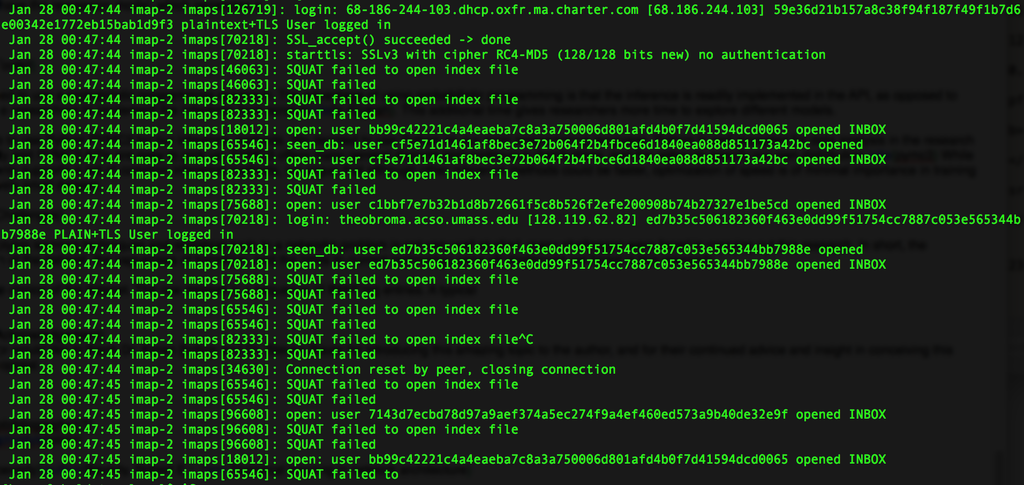
\includegraphics[height = 7cm, width =15cm]{imapSample.png}
 \captionof{figure}{Sample IMAP entry for 2014.01.28}
\end{Figure}

Here we see that the exact ending time for a session is hard to define, unless we see that the connection is reset by peer. In processing our datasets, we made the assumption that a user is on the network unless this network connection is explicitly closed or reset. This can introduce bias for users who were just on the network for a very short period of time but did not detach from the network. We make the argument that from the perspective of network design: since incoming data will still be directed to this idle but attached address, it is reasonable to consider the user as being on the network.

After processing, we have 12 million entries(lines) of sessions, as shown in figure.

\begin{Figure}
 \centering
 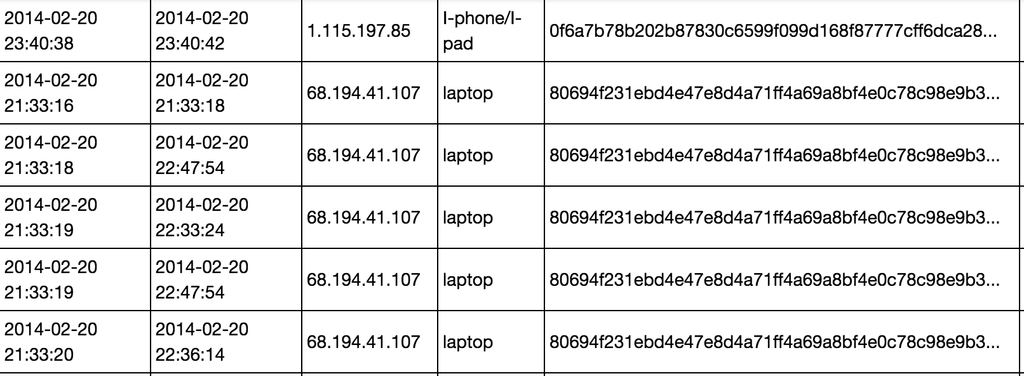
\includegraphics[height = 5cm, width =15cm]{dataSample.png}
 \captionof{figure}{Sample session data, each line is a session. The column headers are session start time, session end time, IP, device, user ID.}
\end{Figure}

This dataset is long but slim, so we went on a pursuit for other relevant features. We included indicator variables for Apple and Android. We included duration of each session, the day of the week, and the city, country, ISP of the IP address. We included an indicator variable for wifi vs. wireless network. Such features were meant to 1. help us achieve higher accuracies in prediction. 2. filter the dataset so that irrelevant data were dropped. While these variables are relevant, none of them is decisively important for our prediction purposes.

One of the major improvements that can happen is to pick a dataset and more carefully process the dataset. The current session definitions have issues regarding end times.

Another aspect of challenge is the technology. We chose to use PYMC3 for our API for probabilistic programming because we believed that probabilistic programming allows for flexibility in creating new models, but this API has its limits. 

One can break down ease of changing models in two cases, here we describe the process with a graphical model approach:

\begin{itemize}
\item
How easy is it to add new features (nodes)?
\item
How easy is it to change the distribution shape of current features (nodes)?
\end{itemize}

For the API we used, it is easy to change the distribution of a feature, but not so much to add a deeply connected node. In PYMC3, we can easily change the shape of the distribution to binomial, normal, Poisson, etc. due to its general inference engine. The NUTS and HMC sampler can easily readapt to the different shapes that we provide as the inference methods were already tuned. For each distribution class, a specific \textit{logp} method is written to facilitate the parameter estimation gradient calculations in NUTS and HMC sampling. Therefore it is very easy to switch models by means of changing distribution.

It is also easy to add new features, as long as the new feature is independent of other features. It is possible to do hierarchical bayesian modeling in PYMC3, but the API was not tuned for hierarchical inference. Working around the API requires hacks that slowed down the progress and incurred bugs that were not informative and difficult to fix. The algorithm returns errors for not being able to infer hierarchically dependent variables. In a neural network, we can specify an extra feature by adding in another column to the input vector / matrix. Even though the nodes can be dependent themselves, the user does not have to specify them. The actual causal dependence is not resolved, but the correlation will be discovered in the hidden layers, by ways of convolutional layers for dimensionality reduction. Such is not possible in PYMC3. We have to specify the graphical model for the variables first. If the parameters are dependent themselves, it is in the user's responsibility to figure out which parameter to infer first. If we change one node, we have to rewrite all other variables that is dependent on that node. This is a particular downside of PYMC3, by providing fast inference through Monte Carlo simulations, it sacrifices flexibility in structural dependency.

Another thing we learnt from applying probabilistic programming techniques is that the model needs to be clearly specified. The human expert needs to know exactly how A and B are linearly, exponentially, or otherwise dependent. In the ideal scenario, once the human feeds in data, the machine magically understand all the hierarchies and dependencies in data on its own, via a selection of possible dependence functions. This belongs to the field of structural learning, which is a more difficult problem. Tenenbaum \cite{tenenbaum} writes on the current state of hierarchical learning. In short, not only is it doing hill climbing in parameter space, but also in modeling space. The current technology seems to have limited grasp on hierarchical structural learning.


\newpage
\section{Acknowledgement}
The author would like to thank Dr. Karen Sollins and Dr. Steven Bauer for introducing this amazing topic to the author, and for their continued advice and insight in conceiving this project and thesis.  This work was funded in part under NSF Grant 1413973, "NeTS: Large: Collaborative Research: Location-Independent Networks: Evaluation Strategies and Studies".



\begin{thebibliography}{7}
\bibliographystyle{plain}
  
\bibitem{beverly}\author{Beverly, Robert E.}. {\em Statistical learning in network architecture}

\bibitem{ghah}\author{Zoubin Ghahramani}. {\em Probabilistic machine learning and artificial intelligence} Nature, 28 May 2015.

\bibitem{jacobson} \author{Jacobson, Van}. {\em Networking Named Content} New York: Association for Computing Machinery, 2009.

\bibitem{ng}\author{Ng, Andrew}. {\em On Discriminative vs. Generative classifiers: A comparison of logistic regression and na�ve Bayes.}

\bibitem{yang}\author{Yang, Sookhyn}. {\em  Measurement and Modeling of User Transitioning Among Networks.}

\bibitem{kulkarni} \author{Kulkarni}. {\em Picture: A Probabilistic Programming Language for Scene Perception.}

\bibitem{find}\emph{NSF NeTS FIND Initiative} http://www.nets-find.net/

\bibitem{pymc3} PyMC3. https://github.com/pymc-devs/pymc3

\bibitem{tenenbaum} \author{Tenenbaum, Joshua}. {\em How to Grow a Mind: Statistics, Structure, and Abstraction.}

\bibitem{tibshirani} \author{Tibshirani, Robert. et al}. {\em Estimating the Number of Clusters in a Data Set via the Gap Statistic.}

\bibitem{ppblog} \author{Finkelstein, Noam}. {\em Probabilistic Programming for Anomaly Detection.}

\bibitem{pymcstan}\author{Carpenter, Bob}. {\em You?ll never guess what's been happening with PyStan and PyMC.}

\bibitem{whyonlyus}\author{Berwick, Rob. Chomsky, Noam}. {\em Why Only Us: Language and Evolution.}

\end{thebibliography}

\end{document}
